\section{Least-Squares Approximation}
\subsection{Linear Least-Squares}
Goal: Approximation of data points by minimizing a function that indicates the deviation in \(y\) (residues).
In this method, the data points are not precisely matched, and the degree \(m\) of the approximation
polynomial is usually significantly smaller than the number of given data points \(N+1\).

From a set of basis functions \(\{g_0, g_1, \ldots, g_m\}\) with \(m \ll N\) and
the measurements \((x_0, y_0), (x_1, y_1), \ldots, (x_N, y_N)\),
the overdetermined (\(m < N\)) system of equations is set up and solved for the unknowns \(a_i\).

\[
    \overbrace{
    \begin{pmatrix}
        g_0(x_0) & g_1(x_0) & \ldots & g_m(x_0) \\
        \vdots & \vdots & \ddots & \vdots \\
        \vdots & \vdots & \ddots & \vdots \\
        g_0(x_N) & g_1(x_N) & \ldots & g_m(x_N)
    \end{pmatrix}}^{\text{Design Matrix } G}
    \cdot
    \begin{pmatrix}
        a_0 \\ \vdots \\ a_m
    \end{pmatrix}
    =
    \begin{pmatrix}
        y_0 \\ \vdots \\ \vdots \\ y_N
    \end{pmatrix}
    \qquad
    \Leftrightarrow
    \qquad
    G \cdot a = y
\]


\begin{minipage}[c]{12.5cm}
	\begin{tabular}{ll}
		Error function to be minimized:
		&$\boxed{\underbrace{S}_{Error}=\sum\limits_{i=0}^{N}{\big(y_i - \underbrace{\sum\limits_{j=0}^{m}{a_j g_j}}_{Model}\big)^2} = \sum\limits_{i=0}^{N}{ r_i^2}}$\\
		Model function:
		&$\boxed{y=\sum\limits_{j=0}^{m}{a_j g_j}}\overset{Poly!}{=}\sum\limits_{j=0}^{m}{a_j x^j}$\\
		Deviations (Residues):
		&$r_i=y_i-\sum\limits_{j=0}^{m}{a_j g_j}$
	\end{tabular}

	\subsubsection{Normal Equation}

	Minimizing the quadratic error with "normal matrix" \(G\) (design matrix):

	$$\underbrace{\bm{G}^T \bm{G}}_{Normal Matrix}\cdot \bm{a} = \bm{G}^T \bm{y} \qquad \Rightarrow \qquad \bm{a}=(\bm{G}^T \bm{G})^{-1}\bm{G}^T \bm{y}$$
	$$\underbrace{\underbrace{\bm{G}^T}_{(m+1)\times(N+1)} \cdot \underbrace{\bm{G}}_{(N+1)\times(m+1)}}_{(m+1)\times(m+1)}\cdot
	  \underbrace{\bm{a}}_{(m+1)\times 1}=
	  \underbrace{\underbrace{\bm{G}^T}_{(m+1)\times(N+1)}\cdot\underbrace{\bm{y}}_{(N+1)\times 1}}_{(m+1)\times 1}$$
\end{minipage}
\hfill
\begin{minipage}[c]{6.5cm}
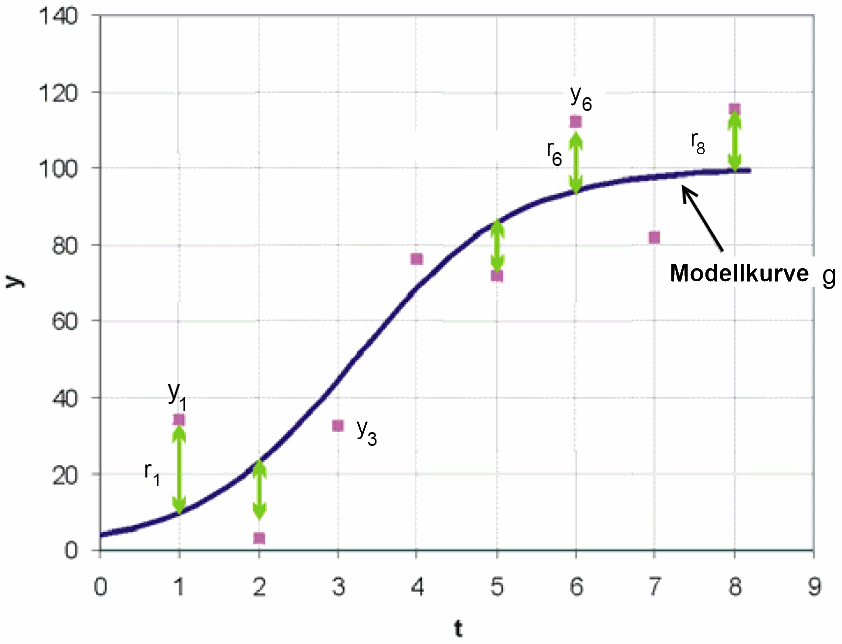
\includegraphics[width=\textwidth]{bilder/leastSquare}\\

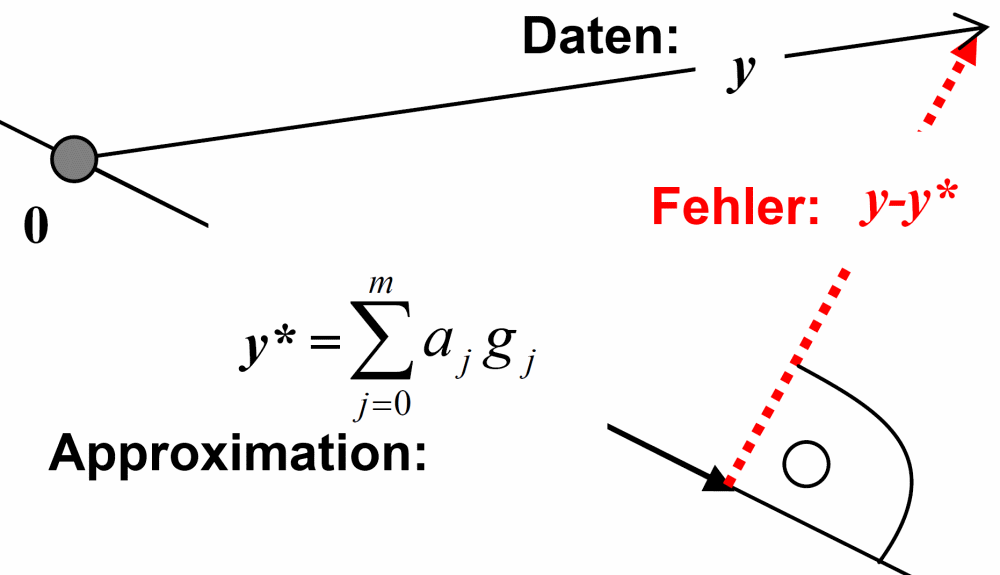
\includegraphics[width=1\textwidth,trim=-3cm 0cm 0cm 0cm]{bilder/leastSquareOrth}
\end{minipage}

The symmetric $(m+1)\times(m+1)$ matrix $G^T \cdot G$ is positive definite if $g_i$ are linearly independent.
The new system of equations is regular and has a unique solution for the coefficients $a_j$.
\[
    \overbrace{
    \begin{pmatrix}
        \langle g_0|,g_0|\rangle & \langle g_1|,g_0|\rangle & \ldots & \langle g_m|,g_0|\rangle \\
        \vdots & \vdots & \ddots & \vdots \\
        \langle g_0|,g_m|\rangle & \langle g_1|,g_m|\rangle & \ldots & \langle g_m|,g_m|\rangle
    \end{pmatrix}
    }^{G^T \cdot G}
    \cdot
    \begin{pmatrix}
        a_0 \\ \vdots \\ a_m
    \end{pmatrix}
    =
    \begin{pmatrix}
        \langle y|,g_0 |\rangle \\ \vdots \\ \vdots \\ \langle y|,g_m| \rangle
    \end{pmatrix}
\]

\subsubsection{QR Decomposition}
A square $n \times n$ matrix $Q$ is orthogonal if $Q^T \cdot Q = Q \cdot Q^T = I$ or $Q^T = Q^{-1}$.
Any matrix $G$ with dimensions $(N+1) \times (m+1)$ where $N \geq m$ and rank $m+1$ can be represented as the product of an orthogonal $(N+1)\times(N+1)$ matrix $Q$ and an upper triangular matrix $R$ with dimensions $(N+1)\times(m+1)$.

The equation system $Ga| = y|$ then becomes $Ra|=Q^Ty|$, which is easier to solve\textsuperscript{Citation needed}.

\subsubsection{Singular Value Decomposition (SVD)}
Any matrix $\bm G$ with dimensions $(N+1) \times (m+1)$ can be decomposed as follows:
$$\bm G = \bm U \bm D \bm V^T = \bm U \cdot \begin{bmatrix}
  d_{00} & 0      & \ldots & 0\\
  0      & d_{11} & \ldots & 0\\
  \vdots & \vdots & \ddots & 0\\
  0      & \ldots & 0      & d_{mm}\\
  0      & 0      & \ldots & 0\\
  \vdots & \vdots & \ddots & 0\\
  0      & 0      & \ldots & 0
\end{bmatrix} \cdot \bm V^T$$
$\bm D$ ($(N+1) \times (m+1)$) is the central diagonal matrix with singular values,
$\bm U$ ($(N+1) \times (N+1)$) and $\bm V$ ($(m+1) \times (m+1)$) are orthogonal and square
matrices (meaning, among other things, that $\bm U^T = \bm U^{-1}$).
The singular values $d_{ii}$ are the square roots of the eigenvalues of $G^T G$,
where the eigenvalues are sorted in descending order.\\

The decomposition itself is not further explained here and can be looked up elsewhere.
SVD can be used to solve equation systems (as here), compute eigenvectors and eigenvalues,
and find inverses.

From $Ga| = y|$ we get $UDV^T a| = y|$. This can be solved to
\[
    a| = V D^{-1}U^T \cdot y|
\]

\subsubsection{Monomials} \label{sssec:ls_monomiale}
With
$g = a_0 \underbrace{1}_{g_0} + a_1 \underbrace{x}_{g_1} + a_2 \underbrace{x^2}_{g_2} +\ldots + a_m \underbrace{x^m}_{g_2}$
the Design Matrix becomes:
\[G \underbrace{=}_{\text{When Monomials}}
\begin{bmatrix}
  1 & x_0 & x_0^2  & \ldots & x_0^m\\
  1 & x_1 & x_1^2  & \ldots & x_1^m\\
  \vdots  & \vdots & \vdots  & \ddots & \vdots\\
  1 & x_N & x_N^2  & \ldots & x_N^m\\
\end{bmatrix}\]


\subsubsection{Uniform Arguments\quad (Orthogonality Properties)} \label{sssec:ls_orthogonal}
With uniform elements $x_i - x_j = (j-i) h$ for all $i, j$ $\rightarrow$ $\{x_0...x_N\} = \{x_0 + t \cdot h\}_{t=0...N}$ and \textbf{orthogonal polynomials},
$G G^T$ can be diagonalized, making the equations computationally simpler to solve.

$$\boxed{p_{k,N}(t) = \sum_{i=0}^k (-1)^i \binom{k}{i} \binom{k+i}{i} \frac{t^{(i)}}{N^{(i)}}=
1+\sum_{i=1}^k (-1)^i \binom{k}{i} \binom{k+i}{i} \frac{t(t-1)(t-2)\ldots(t-i+1)}{N(N-1)(N-2)\ldots(N-i+1)} \qquad (k = 1,\ldots,N)}$$
with $t=\frac{x-x_0}{h} \qquad \binom{k}{i}=\frac{k!}{i!(k-i)!}=nCr(k,i)$\\
$p_{k,N}$ can now be substituted as $g_{k}$ into the design matrix, and the product $G^T G$ becomes
a $(m+1)\times(m+1)$ diagonal matrix. Finally, $a$ can be calculated using the known formula
$G^T G a = G^T y$.

\textbf{Example:}
$$\bm{x}=
	   \begin{bmatrix}
			3&4&5&6&7
	   \end{bmatrix}\qquad \Rightarrow\qquad \bm{t}=\bm{x}-3=
	   \begin{bmatrix}
	   		0&1&2&3&4
	   \end{bmatrix}$$
$$\Rightarrow P_0(x)=1 \qquad P_1(x)= 1-\frac{x-3}{2}\qquad P_2(x)=1-\frac{2\cdot 3 (x-3)}{4}+\frac{1 \cdot 3 (x-3)(x-3 -1)}{4 \cdot 3} = 1-\frac{3x-9}{2}+\frac 12 (x-4)(x-3)???$$
$$\overset{\hspace{0.6cm} P_0 \hspace{0.5cm} P_1 \hspace{0.6cm} P_2}{\bm{G} = \begin{bmatrix}
  1 & 1 	& 1\\
  1 & 1/2 	& -1/2\\
  1 & 0	  	& -1\\
  1 & -1/2 	& -1/2\\
  1 & -1 	& 1\\
\end{bmatrix}}\qquad \Rightarrow\qquad
\bm{G}^T\bm{G}=\begin{bmatrix}
 \| P_0\|^2 	& 0 	& 0\\
  0 		& \|P_1\|^2 	& 0\\
  0 		& 0	  	&\|P_2\|^2\\
\end{bmatrix}
= \begin{bmatrix}
  5 & 0 & 0 \\
  0 & \frac52 & 0\\
  0 & 0 & \frac{7} {2}\\
\end{bmatrix}
$$

\newpage
\subsubsection{Chebyshev Orthogonal Polynomials} \label{sssec:chebyshev_polynom}
\textbf{Idea}: Approximation of a continuous polynomial using Chebyshev polynomials.

\textbf{Definition}\\
Chebyshev polynomials are defined as $\boxed{T_n(x) = \cos(n \arccos(x))}$ with $(n = 0,1,\ldots)$ and $(-1 \leq x \leq 1)$. This
polynomial results in a clustering of data points in the boundary regions. The
first few polynomials $T_n$ and their expressions in terms of $x$:
\begin{tabular}{ll}
  $T_0 = 1$ & $x^0 = 1 = T_0$ \\
  $T_1 = x$ & $x^1 = x = T_1$ \\
  $T_2 = 2x^2 -1$ & $x^2 = \frac12 T_2 + \frac12 T_0$ \\
  $T_3 = 4x^3 - 3x$ & $x^3 = \frac14 T_3 + \frac34 T_1$\\
  $T_4 = 8x^4 -8x^2 + 1$ & $x^4 = \frac18 T_4 + \frac12 T_2 + \frac38 T_0$\\
  $T_5 = 16x^5 - 20x^3 + 5x$ & $x^5 = \frac{1}{16} T_5 + \frac{5}{16} T_3 + \frac58 T_1$\\
\end{tabular}

Additional Chebyshev polynomials can be computed using the recursion formula
$T_{n+1}(x) = 2x T_n(x) - T_{n-1}\; (n\geq2)$
with initial conditions $T_1(x)=x,\;T_0(x)=1$.\\

\textbf{Properties:}
\begin{itemize}
  \item The maximum amplitude of the Chebyshev polynomial is $\frac{1}{2^n}$ (max amplitude of the error term).
  \item Amplitude: $T_n(x) \in [-1,+1]$
  \item Roots: $T_n(x)=0 \Leftrightarrow x=\cos(\frac{2i+1}{2n}\pi)\qquad i=0,1,\ldots,n-1$ (These roots are the Chebyshev nodes)
  \item $T_n(x)= \pm 1 \Leftrightarrow x=\cos(\frac{i\pi}{n}) \; (i=0,1,\ldots,n)$
\end{itemize}

\begin{minipage}{9cm}
  \textbf{Recipe}\\
  Chebyshev polynomials can only be used if \textbf{$x$ with Chebyshev distances}
  $x_i=\cos(\frac{2i+1}{2n}\pi)\;(i=0,1,\ldots,n-1)$ are used and not
  obtained with equidistant distances.

  Goal: Approximate $y(t) = p_N(t)$ (polynomial, defined in $[a,b]$) with Chebyshev polynomials of degree
  $m$.
  \begin{enumerate}
    \item Normalize $y(t)$ to the standard interval $[-1,1]$ (affine transformation)
    $t = a + \frac{b-a}{2} (x+1)$.
    \item Compose $y(x)$ from $T_n$
    \item Truncate $y(x)$ to degree $m$: $y_m(x)$
    \item Back-transform: $x = 2\frac{t-a}{b-a}-1$
    \item Substitute $T_n$ into $y_m$ (see table above)
    \item Error estimate for truncate method:\\
      $\max_{t} |y(t) - y_m(t)|$ (Truncated part)
  \end{enumerate}
\end{minipage}
\hspace{1cm}
\begin{minipage}{9cm}
  \textbf{Example}\\
  Wanted: Approximation $y(t)=t^3$ with degree $m=2$ for interval $(a,b) = (0,1)$
  \begin{enumerate}
  	\item Transformation with $t = \frac{x+1}{2}$:\\
  	  $y(x) = \left( \frac{x+1}{2} \right)^3 = \frac18 (x^3 + 3x^2 + 3x + 1)$
  	\item Expand with table:\\
  	$y(x) = \frac18 \left( \frac{T_3(x) + 3 T_1(x)}{4} + 3 \frac{T_2(x) + T_0}{2} + 3T_1(x) + T_0(x) \right)$\\
  	$=\frac{1}{32}T_3(x) + \frac{3}{16}T_2(x) + \frac{15}{32} T_1(x) + \frac{5}{16}T_0(x)$
  	\item Truncate to degree $m=2$:\\
  	  $y(x) \approx \frac{3}{16}T_2(x) + \frac{15}{32}T_1(x) + \frac{5}{16}T_0(x)$
  	\item Back-transform with $x = 2t-1$:\\
  	  $y(t) \approx \frac{3}{16}T_2(2t-1) + \frac{15}{32}T_1(2t-1) + \frac{5}{16}T_0(2t-1)$
  	\item Replace $T_n(2t-1)$:\\
      $y(t) \approx \frac{3}{16} (2(2t-1)^2-1) + \frac{15}{32}(2t-1) + \frac{5}{16}$
    \item Error estimate:\\
      $\max_t \left| \frac{1}{32}T_3(2t-1) \right|$
  \end{enumerate}
\end{minipage}

\newpage

The \textbf{Design Matrix} looks like this:
$$G \underbrace{=}_{\text{When Chebyshev}}
\begin{bmatrix}
  T_0(x_0) = 1 & T_1(x_0) = x_0 & \ldots & T_m(x_0) \\
  T_0(x_1) = 1 & T_1(x_1) = x_1 & \ldots & T_m(x_1)\\
  \vdots & \vdots  & \ddots & \vdots\\
  T_0(x_N) = 1 & T_1(x_N) =x_N & \ldots & T_m(x_N)\\
\end{bmatrix}_{N \times m}$$

With this, $G^T G$ becomes:
$$G^T G \underbrace{=}_{\text{When Chebyshev}}
\begin{bmatrix}
  N+1 & 0 & \ldots & 0 \\
  0   & \frac{N+1}{2} & \ldots & 0\\
  \vdots  & \vdots & \ddots & \vdots\\
  0   & 0 & \ldots & \frac{N+1}{2}\\
\end{bmatrix}_{m \times m}$$

and $(G^T G)^{-1} G^T$ becomes:

$$(G^T G)^{-1} G^T \underbrace{=}_{\text{When Chebyshev}}
\begin{bmatrix}
  \frac{1}{N+1} T_0(x_0) = \frac{1}{N+1} & \frac{1}{N+1} T_0(x_1) = \frac{1}{N+1} & \ldots & \frac{1}{N+1} T_0(x_N) = \frac{1}{N+1} \\
  \frac{2}{N+1} T_1(x_0) = \frac{2}{N+1} x_0 & \frac{2}{N+1} T_1(x_1) = \frac{2}{N+1} x_1 & \ldots & \frac{2}{N+1} T_1(x_N) = \frac{2}{N+1}x_N\\
  \vdots & \vdots  & \ddots & \vdots\\
  \frac{2}{N+1} T_m(x_0) & \frac{2}{N+1} T_m(x_1) & \ldots & \frac{2}{N+1} T_m(x_N)\\
\end{bmatrix}_{m \times N}$$

\subsubsection{Discrete Least-Squares Chebyshev Approximation}
Follows from $a=(G^T G)^{-1} G^T y$ for $x_i=\cos(\frac{2i+1}{2(N+1)}\pi)\;(i=0,1,\ldots,N)$:
$$p(x) = \sum_{j=0}^m a_j T_j(x) \quad \text{where} \quad
a_j = \begin{cases}
  \frac{1}{N+1} \sum_{i=0}^N y(x_i) & j = 0\\
  \frac{2}{N+1} \sum_{i=0}^N T_j(x_i) y(x_i) & j > 0
\end{cases}$$

\subsubsection{Continuous Least-Squares}
For continuous functions that are \textbf{not polynomials} (!), the continuous version can also be used.\\
S: error function to be minimized, w: weight with ($-1\leq x \leq1$)
\[
	S = \int\limits_{-1}^1 (y(x) - p(x))^2 \cdot w(x) \cdot \mathrm{d}x
\]

\textbf{Continuous Least-Squares Chebyshev Approximation}\\
 The weight is particularly placed on the boundary (as is customary with Chebyshev). ($w(x) = \frac{1}{\sqrt{1-x^2}}$)
$$p(x) = \sum_{j=0}^m a_j T_j(x) \quad \text{where} \quad
a_j = \begin{cases}
  \frac{1}{\pi} \int_{-1}^1 \frac{y(x)}{\sqrt{1-x^2}} dx & j = 0\\
  \frac{2}{\pi} \int_{-1}^1 \frac{y(x) T_j(x)}{\sqrt{1-x^2}} dx & j > 0
\end{cases}$$

\textbf{Continuous Least-Squares Legendre Approximation:}\\
Here, the weight $w(t) = 1$ is used.\\

Legendre Polynomials:
\[
  P_n(x) = \frac{1}{2^n n!} \cdot \frac{\mathrm{d}^n}{\mathrm{d}x^n}(x^2-1)^n \qquad \qquad P_0(x) = 1 \qquad P_1(x) = x \qquad P_2(x) = \frac{1}{2}(3x^2-1)
\]
\[
	  P_3(x) = \frac{1}{2}(5x^3 - 3x) \qquad P_4(x) = \frac{1}{8}(35x^4-30x^2+3) \qquad P_5(x) = \frac{1}{8}(63x^5-70x^3+15x)
\]
\[
	  1 = P_0(x)  \quad x = P_1(x) \quad x^2 = \frac{2P_2(x) + P_0(x)}{3} \quad x^3 = \frac{2P_3(x)+ 3 P_1(x)}{5} \quad x^4 = \frac{8P_4(x) + 20 P_2(x) + 7 P_0(x)}{35} 
\]

Coefficients:
$$
	p(x) = \sum_{j=0}^m a_j P_j(x) \quad \text{wobei} \quad
	a_j = \frac{2j+1}{2} \cdot \int\limits_{-1}^{1}y(x) P_j(x) \cdot \mathrm{d}x \qquad (j=0,1,...,m)
$$

\subsection{Multi-Variate Linear Least Squares Approximation}
Multi-variate least square problems are solved exactly the same way as uni-variate least square problems
(using the same methods)! The variable $x$ is no longer a number but a vector with $d$ dimensions!

\textbf{Basis Generation:}
The bases are computed using the tensor product of uni-variate bases (multiply all with all in d-variables).

\[
	\sum\limits_{j_1=0}^{m_1} \sum\limits_{j_2=0}^{m_2} ... \sum\limits_{j_d=0}^{m_d} a_{j_1,j_2,...,j_d} \cdot g_{j_1}(x^{(1)}) g_{j_2}(x^{(2)}) \cdot \cdot ... \cdot g_{j_d}(x^{(d)})
\]

\paragraph{Examples}
\begin{align*}
    &\text{Basis 3. Grad:} &&
    \{ 1,x,y, \; x^2,2xy,x^2, \; x^3,3x^2y,3xy^2,y^3 \} \\
    &\text{Basis 4. Grad:} &&
    \{ 1,x,y, \; x^2,2xy,x^2, \; x^3,3x^2y,3xy^2,y^3, \; x^4,4x^3y,6x^2y^2,4xy^2,y^4\} \\
\end{align*}

\subsubsection{Matrix Condition Number}
Given a linear system of equations in the form $Ax=b$ with the solution $x = A^{-1} b$.
The condition number $\kappa(A)$ measures the maximum relative error of the solution $x$ with respect to the relative error of the right-hand side $b$:
\[
  \kappa(A) = \begin{cases}
    \max \left(\frac{||\Delta x||/||x||}{||\Delta b|| / ||b||} \quad \text{if } b \neq 0, \Delta b \neq 0, Ax = b\right) & \text{if the matrix } A \text{ is regular}\\
    \infty & \text{otherwise}
  \end{cases}
\]
where $||\ldots||$ denotes a vector norm, usually the Euclidean norm $||\ldots||_2$ or the maximum norm $||\ldots||_\infty$.

If $\kappa (A)$ is relatively small, the system/matrix is called ''well-conditioned,'' otherwise, it is ''ill-conditioned.''

For a regular matrix $A$ and the Euclidean norm $||\dots||_2$:
\begin{itemize}
  \item $\kappa (A) = \frac{|\sigma_{max}|}{|\sigma_{min}|}, \quad |\sigma_{max}| = \text{absolute maximum singular value, and } |\sigma_{min}| = \text{absolute minimum singular value of } A$
  \item If A is also a normal matrix: $\kappa (A) = \frac{|\lambda_{max}|}{|\lambda_{min}|}, \quad |\lambda_{max}| = \text{absolute maximum eigenvalue, and } |\lambda_{min}| = \text{absolute minimum eigenvalue}$
\end{itemize}
